% SIAM Article Template
\documentclass[review,onefignum,onetabnum]{siamart171218}
\usepackage{amssymb}
% Information that is shared between the article and the supplement
% (title and author information, macros, packages, etc.) goes into
% ex_shared.tex. If there is no supplement, this file can be included
% directly.

% SIAM Shared Information Template
% This is information that is shared between the main document and any
% supplement. If no supplement is required, then this information can
% be included directly in the main document.


% Packages and macros go here
\usepackage{lipsum}
\usepackage{amsfonts}
\usepackage{graphicx}
\usepackage{epstopdf}
\usepackage{algorithmic}
\ifpdf
  \DeclareGraphicsExtensions{.eps,.pdf,.png,.jpg}
\else
  \DeclareGraphicsExtensions{.eps}
\fi

% Add a serial/Oxford comma by default.
\newcommand{\creflastconjunction}{, and~}

% Used for creating new theorem and remark environments
\newsiamremark{remark}{Remark}
\newsiamremark{hypothesis}{Hypothesis}
\crefname{hypothesis}{Hypothesis}{Hypotheses}
\newsiamthm{claim}{Claim}

% Sets running headers as well as PDF title and authors
\headers{Movie Recommendation}{N. Grant, R. Guin, T. Hom, S. Qiu}

% Title. If the supplement option is on, then "Supplementary Material"
% is automatically inserted before the title.
\title{Movie Recommendation}

% Authors: full names plus addresses.
\author{Nathan Grant
\and Rudra Guin
\and Tyler Hom
\and Steven Qiu}
  
\usepackage{amsopn}
\DeclareMathOperator{\diag}{diag}


%%% Local Variables: 
%%% mode:latex
%%% TeX-master: "ex_article"
%%% End: 


% Optional PDF information
\ifpdf
\hypersetup{
  pdftitle={Movie Recommendation},
  pdfauthor={N. Grant, R. Guin, T. Hom, S. Qiu}
}
\fi

% The next statement enables references to information in the
% supplement. See the xr-hyperref package for details.

\externaldocument{ex_supplement}

% FundRef data to be entered by SIAM
%<funding-group>
%<award-group>
%<funding-source>
%<named-content content-type="funder-name"> 
%</named-content> 
%<named-content content-type="funder-identifier"> 
%</named-content>
%</funding-source>
%<award-id> </award-id>
%</award-group>
%</funding-group>

\begin{document}

\maketitle

% REQUIRED
\begin{abstract}
In this project we explored various techniques, both used in and out of class to try to accurately predict movie ratings based off of the data set used in lab. Using both techniques used in  and out of class, we used algorithms which preformed very well on the test data.
\end{abstract}

% REQUIRED
\begin{keywords}
  Movie Recommendation, Decision Trees, SVD
\end{keywords}

% REQUIRED
\begin{AMS}
  15A18, 62P20
\end{AMS}

\section{Introduction}
Recommendation systems are some of the most important applications in modern day machine learning. Companies such as Amazon must use purchase history and search trends to predict which items you might want to buy. Netflix faces a similar dilemma in that users will watch and rate movies and they must recommend new movies which the users will like. In this project we explored many approaches to movie recommendation to see what offered the best results.

The biggest challenge to recommendation systems is the sparsity to the data. In the data set any given user only rates a small fraction of the total of movies in the database. Such sparse information makes it hard to make very accurate predictions about what movies the users would enjoy. In our projects we used methods such as Decision Trees, XGBoost, Neural Networks, SVD, and a Weighted SVD Nearest Neighbor approach. 
	We evaluate our results based off of two metrics, accuracy of the classification of a users movie rating, and the mean absolute deviation from the correct rating.

% The outline is not required, but we show an example here.
The paper is organized as follows. Our main results are in
\cref{sec:main}, our new algorithm is in \cref{sec:alg}, experimental
results are in \cref{sec:experiments}, and the conclusions follow in
\cref{sec:conclusions}.

\section{Main results}
\label{sec:main}

The movie recommendation system was evaluated in one of two ways. One way is through human evaluation of the results. Given a user and their rated movies, the algorithm could output movies that they might like. However, this gets tricky because there is no metric to evaluate how good these recommendations actually are. The second option is to take out examples from the training data to use them as test data which was the most promising option. 
First, we approached the problem using classification models where a users data would be input along with the movie data in order to predict what the user would rate the movie. These techniques resulted in accuracies which were not much better than random. 

\Cref{eq:aa} is the first line, and \cref{eq:bb} is the last line.

\section{Algorithm}
\label{sec:alg}

\begin{table}[]
\caption {MAD of Methods Used} \label{tab:title} 
\begin{tabular}{|l|l|}
\hline
Neural Network                & 0.8799 \\ \hline
Regression Tree               & 0.8938 \\ \hline
Random Forest                 & 0.8936 \\ \hline
Gradient Boosted Tree         & 0.8938 \\ \hline
SVD  with Varying KNN         & 0.6326 \\ \hline
SVD with Weighted Varying KNN & .4838\\ \hline
\end{tabular}
\end{table}

\begin{algorithm}
\caption{SVD Nearest Weighted Neighbors}
\label{alg:buildtree}
\begin{algorithmic}
\STATE{Define Epochs: ${1-N}$}
\WHILE{$n < Epochs$}
\STATE{Find $ \triangledown {E = (\frac{\delta E}{\delta W_{i}},...\frac{\delta E}{\delta w_{comp}})}$}
\STATE{Update $W := -\gamma*\triangledown E$ }

\ENDWHILE
\RETURN $W$
\end{algorithmic}
\end{algorithm}


\section{Experimental results}
\label{sec:experiments}

\lipsum[50]

\Cref{fig:testfig} shows some example results. Additional results are
available in the supplement in \cref{tab:foo}.

\begin{figure}[htbp]
  \centering
  \label{fig:a}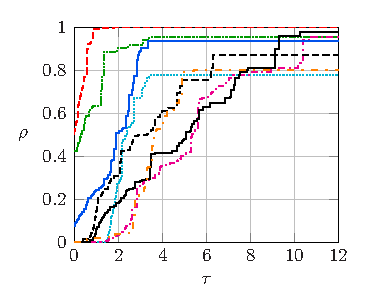
\includegraphics{lexample_fig1}
  \caption{Example figure using external image files.}
  \label{fig:testfig}
\end{figure}

\lipsum[51]

\section{Discussion of \texorpdfstring{{\boldmath$Z=X \cup Y$}}{Z = X union Y}}

\lipsum[76]

\section{Conclusions}
\label{sec:conclusions}

Some conclusions here.


\appendix
\section{An example appendix} 
\lipsum[71]

\begin{lemma}
Test Lemma.
\end{lemma}


\section*{Acknowledgments}
We would like to acknowledge the assistance of volunteers in putting
together this example manuscript and supplement.

\bibliographystyle{siamplain}
\bibliography{references}
\end{document}
